\documentclass{adonis}
\usepackage{hyperref}
\usepackage{tabularx}
\usepackage{xurl}
\usepackage{minted}
\usepackage{graphicx}
\usepackage{fontawesome}


% main details
\title{Generate Answer to Visual Questions in the Medical Domain: Phase 2}
\author{Niki Nezakati - 98522094
\\
\href{https://github.com/nikinezakati/medical-gen-vqa/tree/phase-one}{\faicon{github}} GitHub Repository}




\begin{document}
\definecolor{bg}{rgb}{0.66,0.66,0.66}
	\maketitle
	\section{Creating the Full Sentence Dataset}
	
       In this research, I conducted a study that involved the utilization of the SLAKE dataset, as discussed in phase one. The objective was to generate comprehensive answers from both single and multi-word answers present in the dataset. To accomplish this, I employed the proposed method outlined in the FSVQA article. In order to convert the answers into complete sentences, I leveraged the NLTK language tool and pattern.en part-of-speech tagger. Taking into consideration the relevant question and answer, we applied the language rules introduced in the FSVQA article. A detailed description of these language rules can be found in the table \ref{table1} from this article. By implementing these rules on the SLAKE dataset, we successfully obtained a new dataset comprising answers in the form of complete sentences.
       

       \begin{table}[h]
        \center{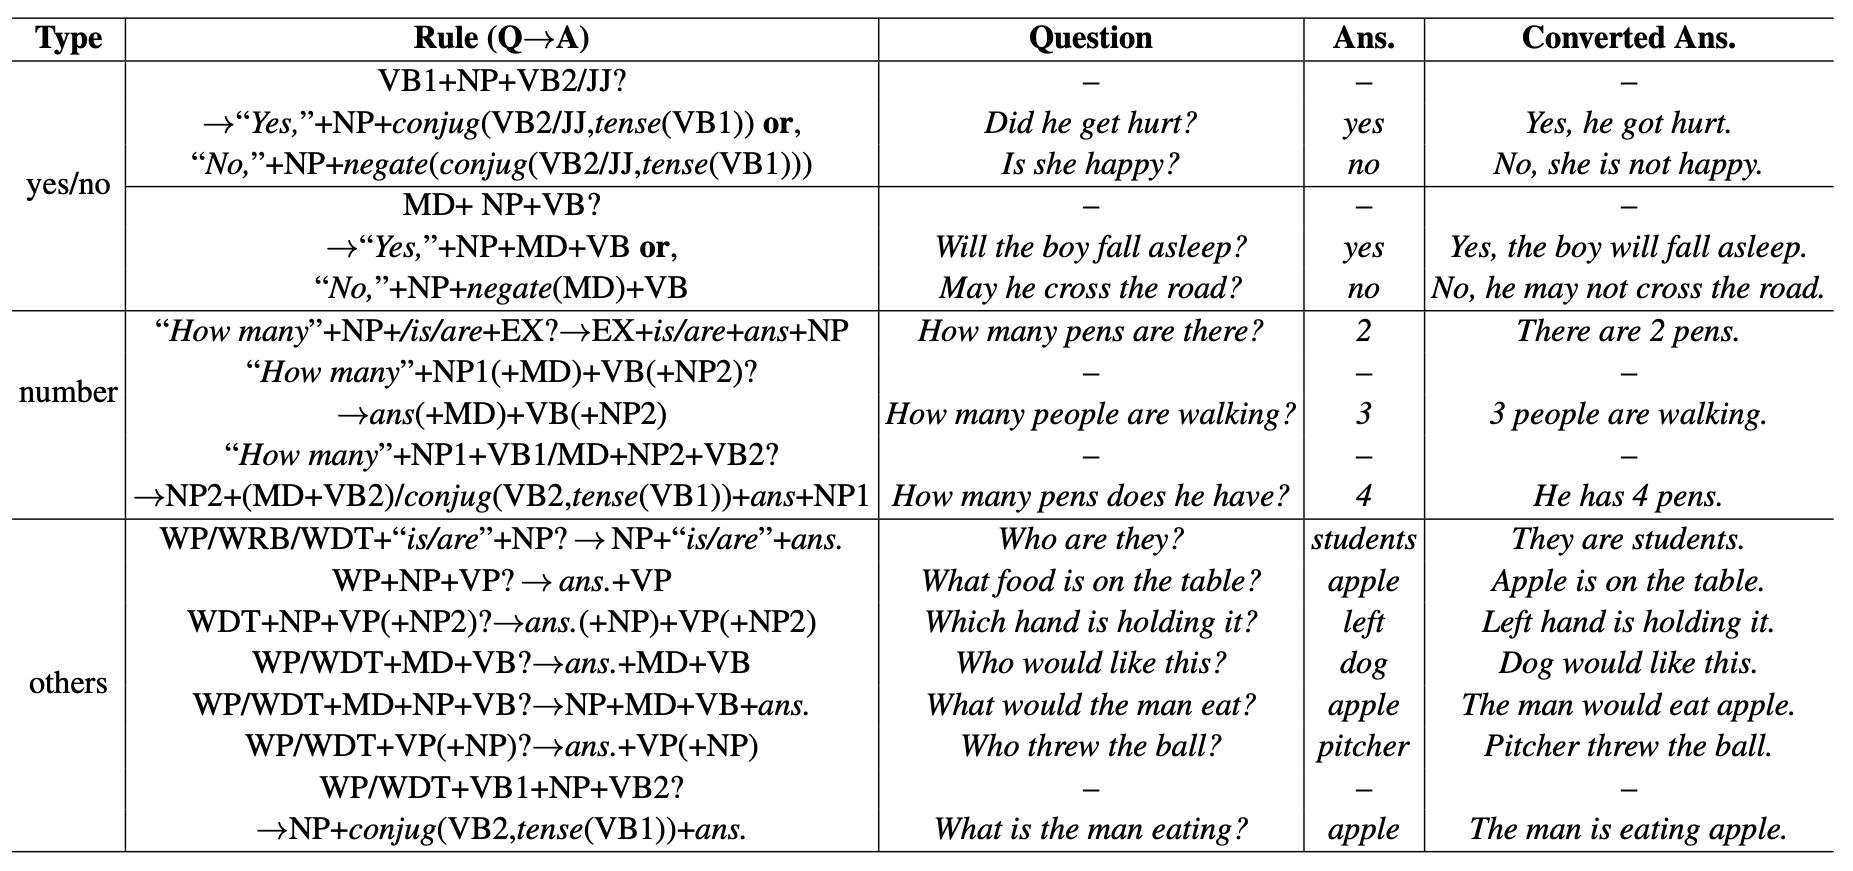
\includegraphics[width=1\textwidth]{images/language-rules.png}}
        \caption{General conversion rules for converting captions to questions.}
    \label{table1}
        % \vspace{-2mm}    
\end{table}

To do this, you should run the bash script located in the run folder named gather\_raw\_data.bash. You can add one argument to this bash which is the output directory and you can specify that or leave it as the default value (data/raw).

        \begin{minted}[bgcolor=bg]{python}
        bash run/gather_raw_data.bash
        \end{minted}

        
  After executing the provided bash script, you will have access to the resulting dataset.  This dataset contains medical images along with corresponding question-answer pairs in both English and Chinese. In the downloaded folder, you will find subfolders containing the images, disease types presented in CSV format, mask file, as well as JSON files for training, validation, and test data. Here is the the amount of instances for each subfolder:



		
		\section{Preprocessing}
	
        To run preprocessing on the data, you should run the bash script located in run folder with name preprocess\_raw\_data.bash. You can add one argument to this bash which is the output directory and you can specify that or leave it as the default value (data/preprocessed).
        \begin{minted}[bgcolor=bg]{python}
        bash run/preprocess_raw_data.bash
        \end{minted}

        
  This preprocessing step selects the English data which will be used in the project. This is done by selecting dictionary instances that have the key-value pair of ['q\_lang'] == 'en' in the JSON files for training, validation, and test data. The resulted data is saved as JSON files for training (4919 instances), validation (1053 instances), and test (1053 instances) data. Here is the the amount of instances for each subfolder:

   \begin{table}[H]
  \centering
  \setlength{\tabcolsep}{1.5em}
  {\renewcommand{\arraystretch}{1.2}
    \begin{minipage}{15.5cm}
  \begin{tabular}{ | l | c | r | }
    \hline
    English Train Data & English Validation Data & English Test Data \\ \hline
    4919 & 1053 & 1061 \\ \hline
  \end{tabular}
  \end{minipage}}
  \end{table}

  \section{Tokenization}
	
        To run tokenization on the English data, you should run the bash script located in run folder with name break\_data.bash. You can add two arguments to this bash which are the output directory for word and sentence tokenization. You can specify that or leave it as the default value (data/wordbroken) and (data/sentencebroken).
        \begin{minted}[bgcolor=bg]{python}
        bash run/break_data.bash
        \end{minted}

  This step involves tokenizing the English questions and answers into individual words and sentences. Word tokenization is done by splitting the English questions and answers by punctuation marks. In the sentence tokenization process, we include each question individually since they consist of only one sentence. The resulted data is saved as JSON files for training, validation, and test data. Here is the the amount of instances for each subfolder:


  \begin{table}[H]
  \centering
  \setlength{\tabcolsep}{0.7em}
  {\renewcommand{\arraystretch}{1.2}
    \begin{minipage}{15.5cm}
    \begin{tabular}{ | l | c | r | }
    \hline
    Train Question Words & Validations Question Words & Test Question Words \\ \hline
    39573 & 8868 & 8722 \\ \hline
  \end{tabular}
  \end{minipage}}
  \end{table}



\begin{table}[H]
  \centering
  \setlength{\tabcolsep}{0.8em}
  {\renewcommand{\arraystretch}{1.2}
    \begin{minipage}{15.5cm}
  \begin{tabular}{ | l | c | r | }
    \hline
    Train Question Sents. & Validations Question Sents. & Test Question Sents. \\ \hline
    4919 & 1053 & 1061 \\ \hline
  \end{tabular}
  \end{minipage}}
  \end{table}


\begin{table}[H]
  \centering
  \setlength{\tabcolsep}{0.9em}
  {\renewcommand{\arraystretch}{1.2}
    \begin{minipage}{15.5cm}
  \begin{tabular}{ | l | c | r | }
    \hline
    Train Answer Words & Validations Answer Words & Test Answer Words \\ \hline
    6912 & 1537 & 1558 \\ \hline
\end{tabular}
  \end{minipage}}
  \end{table}


 \section{Statistics}
 To run Statistics on the English data, you should run the bash script located in run folder with name stats.bash.
        \begin{minted}[bgcolor=bg]{python}
        bash run/stats.bash
        \end{minted}

This step involves finding unique answer (words), and questions (sentences) in train, validation, and test labels. We categorize them by the common ones (unique words that appear in more than one label), or uncommon ones. The code was designed to generate a count of word and sentence occurrences. The resulted data is saved as CSV files for training, validation, and test data. Here is the the amount of instances for each subfolder:  


\begin{table}[H]
  \centering
  \setlength{\tabcolsep}{0.4em}
  {\renewcommand{\arraystretch}{1.2}
    \begin{minipage}{15.5cm}
  \begin{tabular}{ | l | c | r | }
    \hline
    Unique Train Questions & Unique Validation Questions & Unique Test Questions \\ \hline
    597 & 318 & 319 \\ \hline
\end{tabular}
  \end{minipage}}
  \end{table}

Bellow are the count of individual words in questions and answers:

\begin{table}[H]
  \centering
  \setlength{\tabcolsep}{0.4em}
  {\renewcommand{\arraystretch}{1.2}
    \begin{minipage}{15.5cm}
  \begin{tabular}{ | l | c | r | }
    \hline
    Unique Train Questions & Unique Validation Questions & Unique Test Questions \\ \hline
    284 & 245 & 252 \\ \hline
\end{tabular}
  \end{minipage}}
  \end{table}


  \begin{table}[H]
  \centering
  \setlength{\tabcolsep}{0.7em}
  {\renewcommand{\arraystretch}{1.2}
    \begin{minipage}{15.5cm}
  \begin{tabular}{ | l | c | r | }
    \hline
    Unique Train Answers & Unique Validation Answers & Unique Test Answers \\ \hline
    275 & 191 & 189 \\ \hline
\end{tabular}
  \end{minipage}}
  \end{table}


  \begin{table}[H]
  \centering
  \setlength{\tabcolsep}{0.19em}
  {\renewcommand{\arraystretch}{1.2}
    \begin{minipage}{15.5cm}
  \begin{tabular}{ | l | c | r | }
    \hline
    Common Uniq. Train Ans. & Common Uniq. Valid Ans. & Common Uniq. Test Ans. \\ \hline
    230 & 137 & 139 \\ \hline
\end{tabular}
  \end{minipage}}
  \end{table}



  \begin{table}[H]
  \centering
  \setlength{\tabcolsep}{0.5em}
  {\renewcommand{\arraystretch}{1.2}
    \begin{minipage}{15.5cm}
  \begin{tabular}{ | l | c | r | }
    \hline
    Uncom. Uniq. Train Ans. & Uncom. Uniq. Valid Ans. & Uncom. Uniq. Test Ans. \\ \hline
    45 & 54 & 50 \\ \hline
\end{tabular}
  \end{minipage}}
  \end{table}

  
\newpage
\vspace{10pt}
  Finally, the histograms displayed below represent the frequency of occurrence for the top 20 most unique label tokens, considering the large number of distinct tokens involved in the answers.
  
 \begin{center}
       \hspace*{-1.5cm}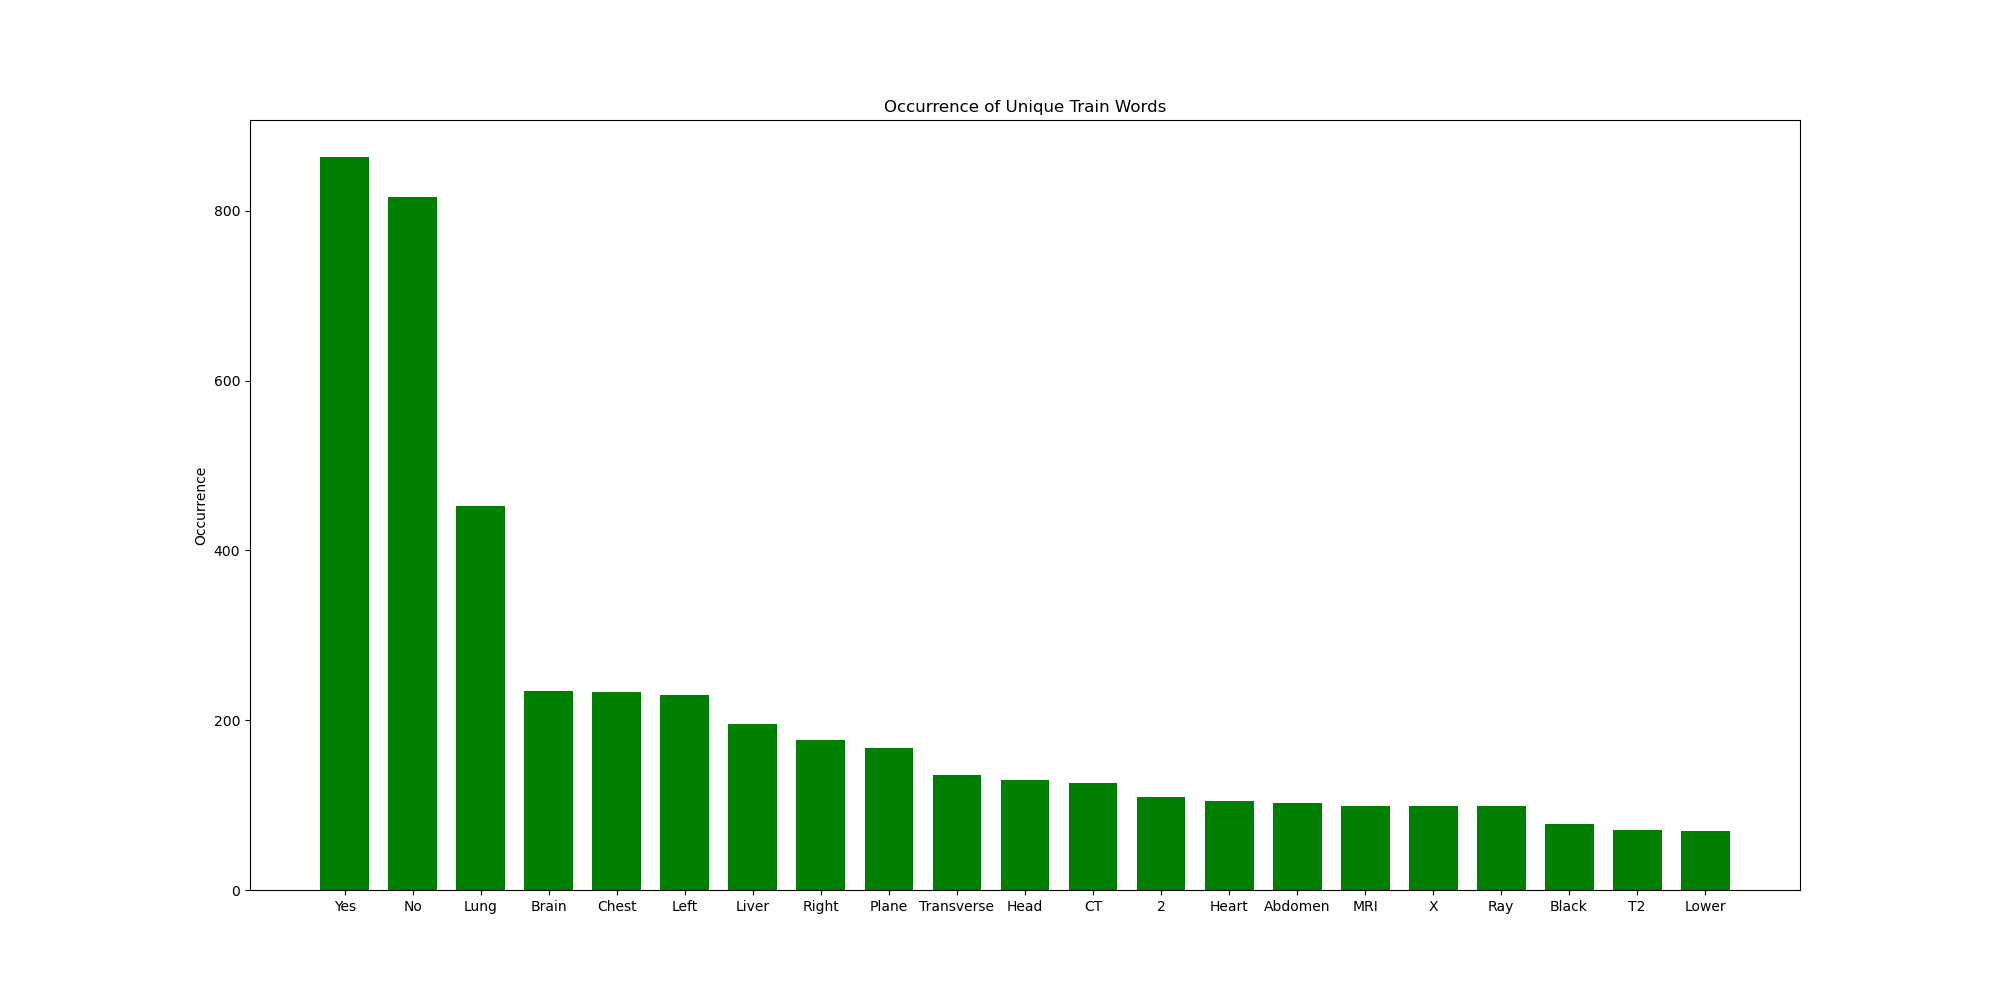
\includegraphics[width=15cm]{images/train_unique_words.png}
\end{center}


    \begin{center}
         \hspace*{-1.5cm}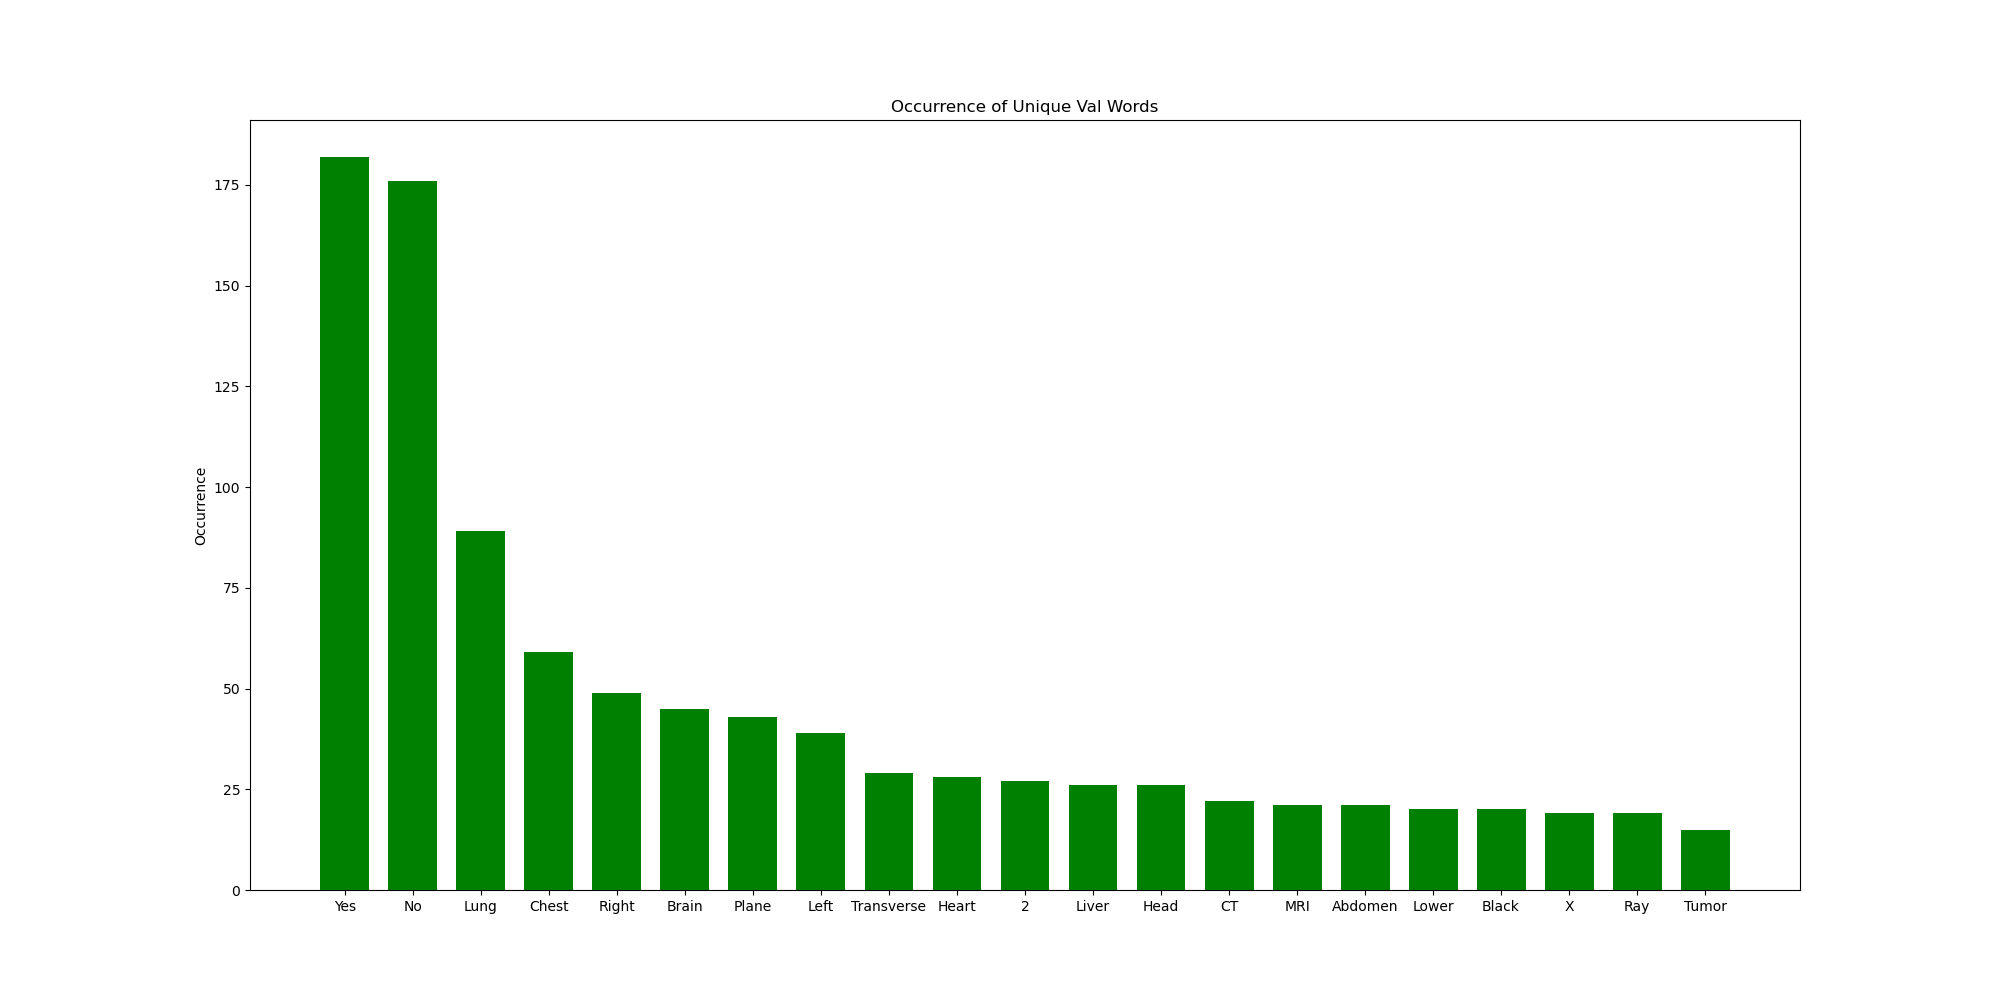
\includegraphics[width=15cm]{images/val_unique_words.png}
\end{center}


    \begin{center}
         \hspace*{-1.5cm} 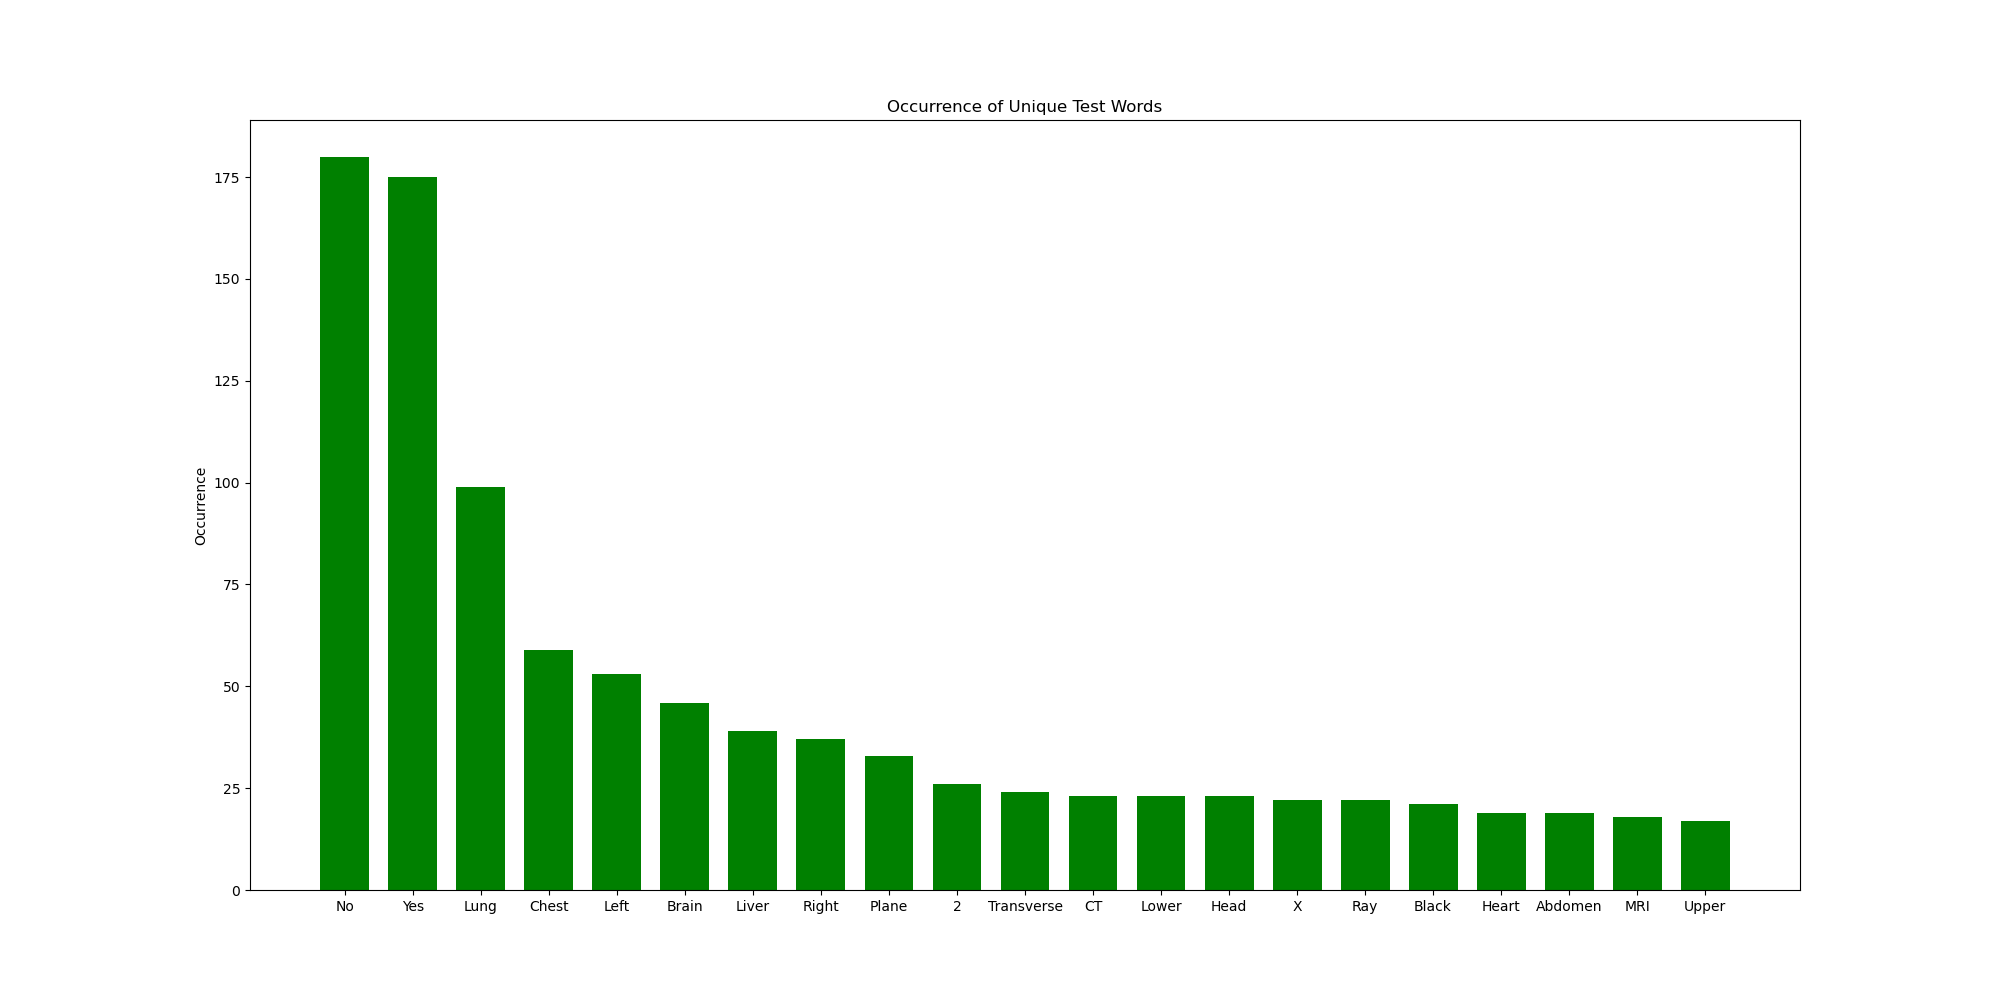
\includegraphics[width=15cm]{images/test_unique_words.png}
\end{center}

Note that due to the nature of the labels being comprised of single or multiple distinct words, it is not meaningful to assess measures such as the frequency of occurrence of label tokens, or identifying the most commonly appearing words.



 
	% \section{Layout}
	
	% 	The \textit{Adonis} template is based on the base \textit{article} template.
	% 	To use the template, you need to copy the \verb+adonis.cls+ class file to the same directory as your manuscript.
	% 	Then, specify the document class in the preamble:
		
	% 	\begin{verbatim}
	% 		\documentclass[twocolumn]{adonis}
	% 	\end{verbatim}
		
	% 	The paper dimensions are those of an A4 paper.
	% 	Many changes concern its layout, and most add white space.
	% 	The margins are wider, notably on the sides, but also at the top and bottom.
	% 	The extra space serves a dual purpose: an obvious aesthetic one, and a more functional one.
	% 	The wider margins afford margin notes more space, and thus gives them more prominence.
		
	% 	Unlike the \textit{article} template, \textit{Adonis} includes a header and a footer, albeit in small print.
	% 	The header shows the running author on the left and the running title on the right, while the footer shows the page number in the centre.
	% 	You can specify the running author and title as follows:
		
	% 	\begin{verbatim}
	% 		\runningauthor{Yours truly et al.}
	% 		\runningtitle{Short title}
	% 	\end{verbatim}
		
	% 	If you do not define them, the template uses the author and title fields instead.
	% 	\textit{Adonis} does not show the header and footer on the first page, which is already busy.
		
	% 	\subsection{Options}
		
	% 		The \textit{Adonis} template comes with optional directives to change how the manuscript looks.
	% 		By default, the template has one column and wide margins, but you can change both.
	% 		Remember that you can use multiple options, or none at all.
			
	% 		\subsubsection{Dark mode}
			
	% 			The dark mode sets a the page colour to a dark grey and the text to white to reduce eye strain during writing sessions.
	% 			To enable dark mode, pass the \texttt{dark} option to the \textit{Adonis} template:
				
	% 			\begin{verbatim}
	% 				\documentclass[dark]{adonis}
	% 			\end{verbatim}
			
	% 		\subsubsection{Legacy}
			
	% 			The legacy layout adds backwards compatibility for old packages.
	% 			Specifically, the legacy layout does not load the \texttt{notomath} package, which the template uses to render mathematical text.
	% 			Use the legacy layout on versions of TeX Live from before 2021, which do not include the package.
	% 			To enable the legacy layout, pass the \texttt{legacy} option to the \textit{Adonis} template:
				
	% 			\begin{verbatim}
	% 				\documentclass[legacy]{adonis}
	% 			\end{verbatim}
		
	% 		\subsubsection{Two columns}
			
	% 			The two-column layout gives the manuscript a conference paper-like look.
	% 			Since a two-column layout takes up more space, \textit{Adonis} reduces the margin sizes.
	% 			Part of the reclaimed margin size goes to the column separation to give the document a clean look and improve readability.
	% 			To enable the two-column layout, pass the \texttt{twocolumn} option to the \textit{Adonis} template:
			
	% 			\begin{verbatim}
	% 				\documentclass[twocolumn]{adonis}
	% 			\end{verbatim}
			
	% 		\subsubsection{Wide}
			
	% 			The default layout has wide margins, both to give the document a clean look and to reserve more space for margin notes.
	% 			If you require neither, you can reduce margin space and widen the text area by using the wide option:
			
	% 			\begin{verbatim}
	% 				\documentclass[wide]{adonis}
	% 			\end{verbatim}
	
	% 	\subsection{Front-matter}
		
	% 		\textit{Adonis} changes the \textit{article}'s front page to make a better first-impression.
	% 		The title is no longer centred nor justified, and in the two-column layout, it occupies only one column.
	% 		Moreover, to give the title more prominence, the template shrinks secondary information and moves some of it to the bottom of the page.
	% 		The template thus splits the front-matter into two parts, the main and secondary details.
			
	% 		\subsubsection{Main details}
			
	% 		The main details include three parts: the title, the author and the abstract.
	% 		To make the difference evident, the template gives the title a large font size and the author a smaller size, and italicizes the abstract.
	% 		A horizontal rule separates the abstract from the main content.
			
	% 		In the two-column layout, \textit{Adonis} also starts a new column after the abstract.
	% 		The white-space gives the template character and increases the separation between the abstract and the main text.
	% 		The title also appears slightly smaller in two-column layout, again due to the decreased space.
	% 		You can specify the title, author and abstract using dedicated commands:
			
	% 		\begin{verbatim}
	% 			\title{Your title}
	% 			\author{Yours truly}
	% 			\abstract{\lipsum[0]}
	% 		\end{verbatim}
			
	% 		\subsubsection{Secondary details}
			
	% 		The rest of the front-matter details, including the affiliations, the date of publication and the correspondence, appear at the bottom of the page in small type.\footnote{
	% 			To keep the template as simple as possible, \textit{Adonis} does not match the author with the affiliations.
	% 			In other words, you need to link the author with the affiliations manually, such as by adding superscript numbers next to your authors and next to their affiliations.
	% 		}
	% 		The secondary details are separated from the abstract and main text by a horizontal rule.
	% 		The template only renders the secondary details if you fill them in explicitly, so if you need a quick-start, you can leave them out altogether.
	% 		You can specify the secondary details using dedicated commands:
			
	% 		\begin{verbatim}
	% 			\affiliation{Affiliation}
	% 			\correspondence{youremail@tld.com}
	% 			\date{\today}
	% 		\end{verbatim}
		
	% \section{Typography}
	
	% 	The second major change concerns the typography.
	% 	\textit{Adonis} uses the Source font family to improve readability: Source Serif Pro for the main text, and Source Sans Pro for headings.
	% 	All paragraphs are justified to give the document a clean look.
		
	% 	\textit{Adonis} uses the same font size as in the base \textit{article} template: 10pt.
	% 	Differently from it, however, \textit{Adonis} uses a larger line-height: 1.4.
	% 	Apart from the normal size, the template also defines the \texttt{tiny}, \texttt{footnotesize}, \texttt{small}, \texttt{large} and \texttt{huge} sizes.
	% 	Font sizes larger than normal use a smaller line-height: about 1.2.
		
	% 	Moreover, \textit{Adonis} makes some subtler changes.
	% 	For example, the template uses the semi-bold font-weight in place of the actual bold-weight when using \texttt{\textbackslash{}textbf}, which looks more subtle next to the regular font-weight.
	% 	The template also uses the \texttt{microtype} package to enable protrusion and expansion; the former lets punctuation bleed slightly into the margins, and the latter uses varying font widths to make the word-spacing more even.
		
		% \subsection{Math}
		
		% 	The Source Pro family does not have support for mathematical text.
		% 	Instead, \textit{Adonis} uses the Noto Serif font to render mathematical text.
		% 	For example, the following equation represents the golden ratio $\phi$, on which I based the page margins.
		% 	The font has a thickness much closer to Source Serif's than the default font.
		
		% 	\begin{equation}
		% 		\phi = \frac{1 + \sqrt{5}}{2}
		% 	\end{equation}
		
		% 	Note that the \texttt{notomath} package is only available from TeX Live 2021 onward.
		% 	To use the template on earlier versions, pass the \texttt{legacy} option to the document class:
			
		% 	\begin{verbatim}
		% 		\documentclass[legacy]{adonis}
		% 	\end{verbatim}

		% \subsection{Headings}
		
		% 	Unlike the rest of the text, headings use the Source Sans Pro family.
		% 	All headings have the same size as the text, but they have a semi-bold font-weight and a small-caps shape.
		% 	The different font serves to draw attention to headings, and thus make the manuscript easier to navigate.
		% 	\textit{Adonis} supports three heading levels.
		
		% 	\subsubsection{Section}
			
		% 		The section is the highest level in manuscripts.
		% 		Therefore \textit{Adonis} adds a hefty margin before them, such that sections leap out when scrolling.
			
			
			
			
	% \section{Other elements}
	
	% 	\begin{table*}[t!]
	% 		\begin{tabularx}{\linewidth}{ l l X }
	% 			\textbf{Version} & \textbf{Date} & \textbf{Changelog} \\ \hline
	% 			0.1 & April 16, 2023 & Initial release \\
	% 			0.2 & May 12, 2023   & Improved text readability, new math font and \texttt{legacy} option, dark mode, and miscellaneous layout changes \\
	% 		\end{tabularx}
	% 		\caption{The template's version history.}
	% 		\label{"Table: version history"}
	% 	\end{table*}
	
	% 	In addition to the layout and typography, \textit{Adonis} also makes slight changes to other common \LaTeX{} elements.
	% 	The template gives table cells more padding and rows more space, as shown in Table~\ref{"Table: version history"}.

	% 	Margin notes also use a smaller font size such that they are not too prominent.
	
	
	\begin{thebibliography}{5}
		\bibitem{slake}
		SLAKE: A Semantically-Labeled Knowledge-Enhanced Dataset for Medical Visual Question Answering. Bo Liu, Li-Ming Zhan, Li Xu, Lin Ma, Yan Yang, Xiao-Ming Wu (2021). \url{https://arxiv.org/abs/2102.09542}
	\end{thebibliography}
	
\end{document}